\documentclass[a4paper, 12pt, final, garamond]{book}
\usepackage{cours-preambule}

\raggedbottom

\makeatletter
\renewcommand{\@chapapp}{M\'ecanique -- chapitres}
\renewcommand\thechapter{6 et 7}
\makeatother

\begin{document}
% \setcounter{chapter}{0}

\chapter{TD~: moment cin\'etique et forces centrales}

\section{Gravimètre de \textsc{Holweck-Lejay}}

Une masse ponctuelle $m$ est placée à l'extrémité M d'une tige de masse
négligeable et de longueur $L = \OMr$, articulée en O et mobile dans un plan
vertical. Un ressort «~spirale~» (non représenté sur la figure) exerce sur M,
via la tige, un couple de rappel (notion abordée au chapitre 8) équivalent à un
moment de force dont la projection sur $(\Or z)$ est $\Mc_z = -C\tt$ avec $C>0$.

\begin{minipage}[]{0.25\linewidth}
    \begin{center}
        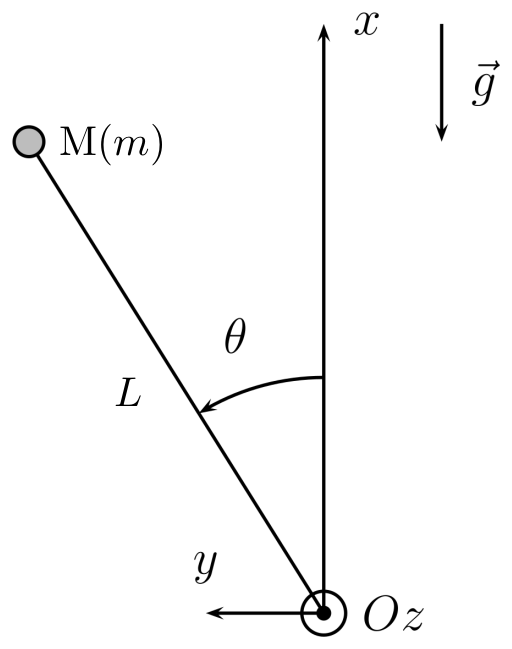
\includegraphics[width=\linewidth]{holweck-plain_m}
    \end{center}
\end{minipage}
\hfill
\begin{minipage}[]{0.70\linewidth}
    \begin{enumerate}
        \item Déterminer, par l'application du théorème du moment cinétique par
            rapport à l'axe $(\Or z)$, l'équation différentielle vérifiée par
            $\tt$.
        \item À l'aide d'un développement de \textsc{Taylor} autour de $\tt =
            0$, déterminer la condition sur $C$ pour que $\tt = 0$ soit une
            position d'équilibre stable.
        \item Retrouver ce résultat en établissant l'énergie potentielle du
            ressort spiral puis en étudiant la stabilité par une approche
            énergétique.
        \item À partir de l'équation différentielle simplifiée à la question 2,
            calculer la période $T$ des petites oscillations autour de $\tt =
            0$.
        \item En posant $g_0 = C/mL$, déduire des résultats précédents une
            méthode de mesure de $g$.
    \end{enumerate}
\end{minipage}

\section{Frottements d'un satellite}
\begin{wrapfigure}[5]{R}{.20\linewidth}
    \vspace*{-10pt}
    \centering
    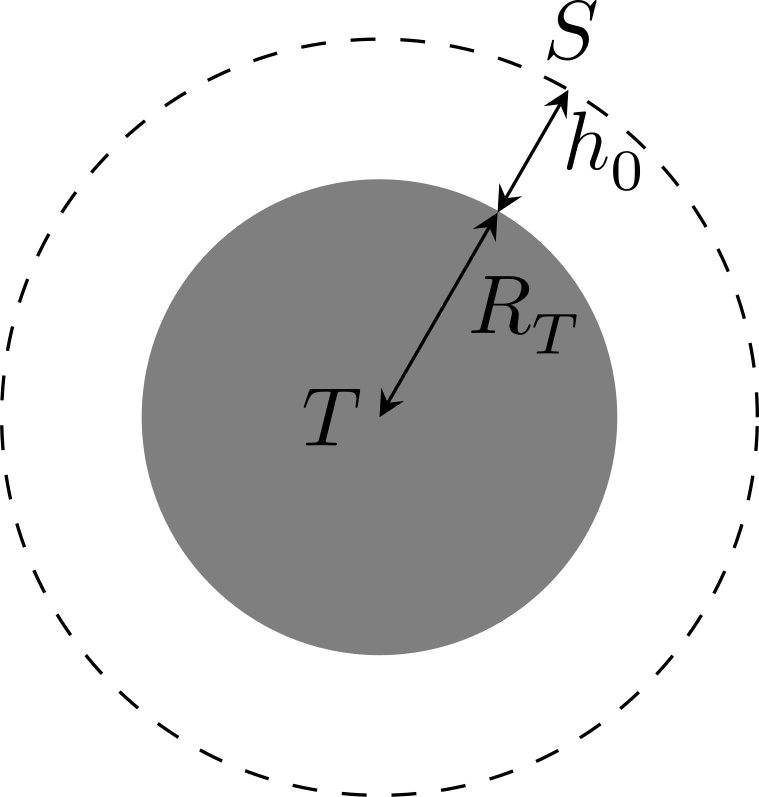
\includegraphics[width=\linewidth]{frott_sat-plain}
\end{wrapfigure}
Un satellite S de masse $m$ décrit une trajectoire circulaire uniforme
d'altitude $h_0$ autour de la Terre de masse $m_T$ et de rayon $R_T$, dans le
référentiel géocentrique.

\begin{enumerate}
    \item Exprimer la norme $v$ de son vecteur vitesse et son énergie mécanique
        $\Ec_m$ en fonction de $\Gc$, $m_T$, $m$, $R_T$ et $h_0$. On pourra
        localement introduire $R=R_T+h_0$.
    \item Le satellite étant sur une orbite basse, il subit de la part des
        hautes couches de l'atmosphère une force de frottements qui modifie son
        altitude $h$. Cependant, \textbf{on considère que la trajectoire sur un
        tour reste quasi-circulaire}~; ainsi les expressions précédentes restent
        valables en remplaçant $h_0$ par $h(t)$.
        \begin{enumerate}
            \item Le travail des forces de frottements est-il moteur ou
                résistant~? En déduire le signe de $\dv{\Ec_m}{t}$.
            \item Comment évolue le rayon de l'orbite du satellite au cours du
                temps~? Tracer l'allure de sa trajectoire.
            \item En déduire le sens de variation de la vitesse. Commenter.
        \end{enumerate}
\end{enumerate}

\section{Pendule conique}

\begin{minipage}{0.70\linewidth}
    Dans un champ uniforme de pesanteur $\gf$ vertical et vers le bas, un point
    matériel M de masse $m$ tourne à la vitesse angulaire $\w$ constante autour
    de l'axe $(\Or z)$, dirigé vers le haut, et décrit ainsi un cercle de centre
    O et de rayon $R$. M est suspendue à un fil inextensible de longueur $L$ et
    de masse négligeable, fixé en un point A de $(\Or z)$. L'angle $\a$ de $(\Or
    z)$ avec AM est constant. \smallbreak On travaille dans le référentiel du
    laboratoire supposé galiléen. On utilisera le repère de la base cylindrique
    tel que $\OM = R\ur$.
\end{minipage}
\begin{minipage}{0.25\linewidth}
    \begin{center}
        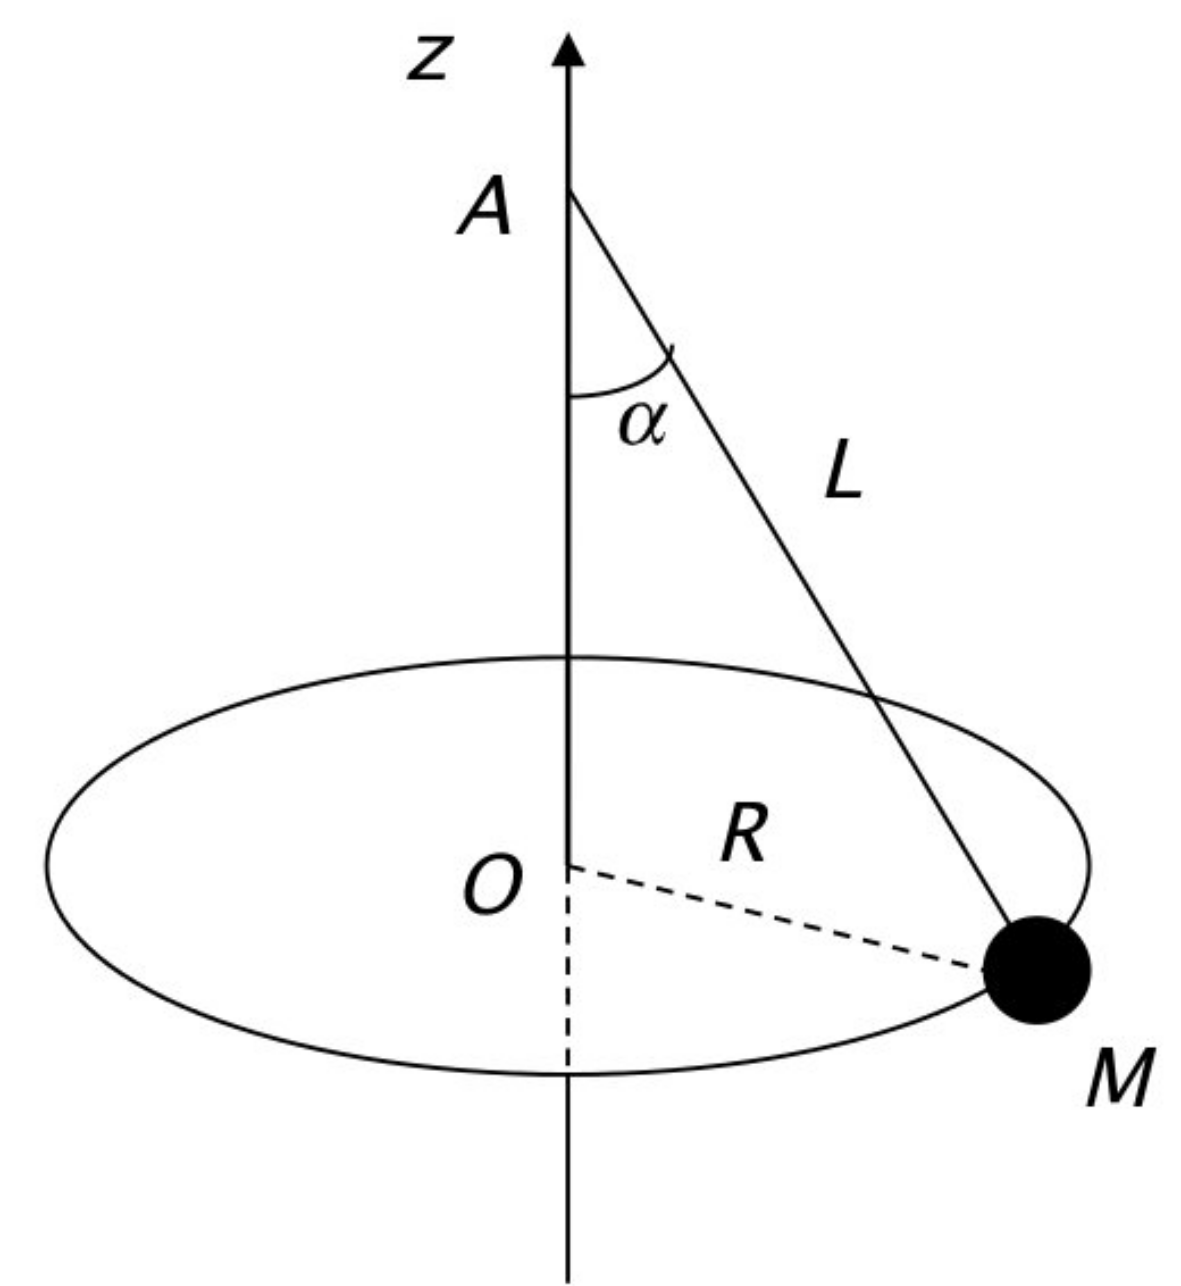
\includegraphics[width=\linewidth]{pendule_conique-plain}
    \end{center}
\end{minipage}

\begin{enumerate}
    \item Exprimer le moment cinétique de M par rapport à A en fonction de $m$,
        $M$, $\w$ et $\a$.
    \item Appliquer le TMC pour déduire $\cos\a$ en fonction de $g$, $L$ et
        $\w$.
    \item Retrouver ce résultat à partir du PFD.
\end{enumerate}

\section{Comète de \textsc{Halley}}

\begin{minipage}{0.70\linewidth}
    La comète de \textsc{Halley} est la plus connue. La première mention de son
    observation date de 611 av. J.-C.\ en Chine, et on la retrouve tout au long
    de l'Antiquité et du Moyen Âge, évidemment sans savoir qu'il s'agit d'une
    seule comète. Cette découverte a été formalisée en 1705 par Edmond
    \textsc{Halley,} qui publia un livre avançant que les observations en 1531,
    1607 et 1682 concernaient en fait la même comète. Son prochain passage est
    prévu en 2061. On sait aujourd'hui que la comète de \textsc{Halley} suit une
    trajectoire elliptique de période de révolution autour du Soleil 76 ans, sa
    distance minimale au Soleil étant de $d_{\min} = \SI{0.59}{UA}$.
\end{minipage}
\hfill
\begin{minipage}{.25\linewidth}
    \begin{center}
        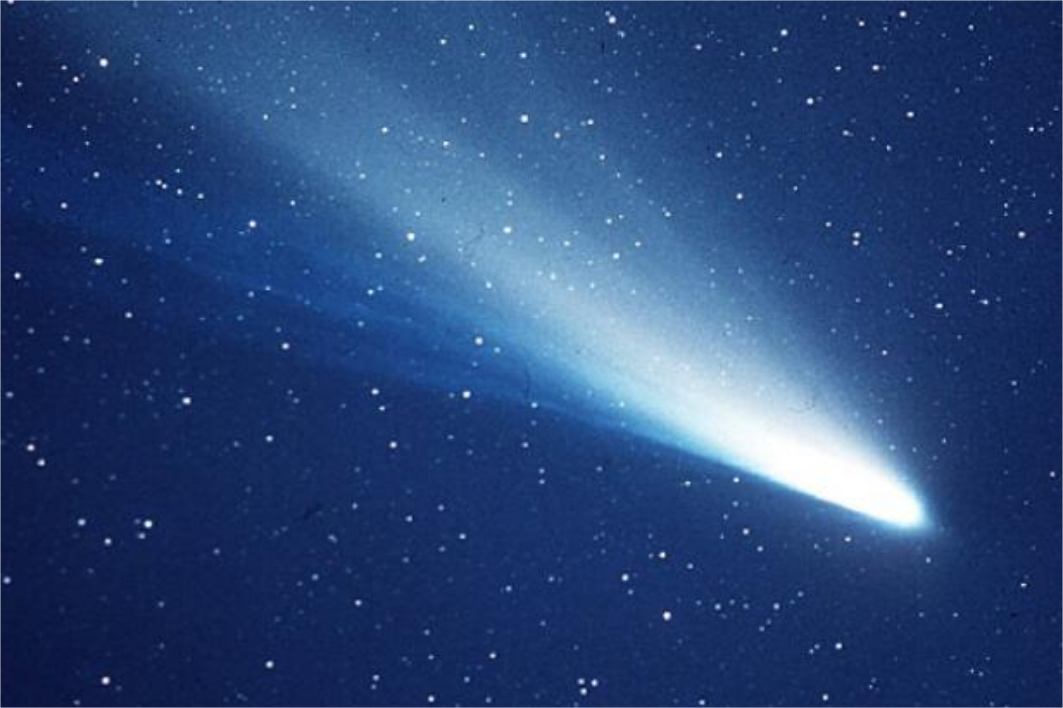
\includegraphics[width=\linewidth]{halley}
    \end{center}
\end{minipage}
\begin{rdefi}{Données}
    \begin{itemize}
        \item Masse solaire $m_S = \SI{2.0e30}{kg}$.
        \item UA signifie «~unité astronomique~», et correspond à la distance
            moyenne entre la Terre et le Soleil. $\SI{1}{UA} = \SI{1.5e11}{m}$.
    \end{itemize}
\end{rdefi}

\begin{enumerate}
    \item Faire un schéma de la trajectoire de la comète en faisant aussi
        apparaître la position du Soleil et $d_{\min}$.
    \item Déduire de la troisième loi de \textsc{Kepler} la plus grande distance
        de la comète au Soleil.
    \item Une conique est décrite par une équation polaire de la forme
        \[r(\tt) = \frac{p}{1-e\cos\tt}\]
        où l'origine du repérage polaire est prise sur un des foyers de la
        conique. Déterminer le paramètre $p$ et l'excentricité $e$ de la
        trajectoire de la comète de \textsc{Halley}.
\end{enumerate}

\section{Changement d'orbite}

\begin{minipage}{0.70\linewidth}
    Un satellite artificiel assimilé à un point matériel M de masse $m_s$ trouve
    sur une orbite circulaire provisoire de rayon $r_1 = \SI{7500}{km}$ autour
    de la Terre. On souhaite le faire passer sur son orbite définitive de rayon
    $r_2 = \SI{42200}{km}$ (orbite géostationnaire). Pour cela, on le fait
    d'abord passer sur une orbite de transfert elliptique dont le périgée P est
    à la distance $r_1$ et l'apogée A à la distance $r_2$ du centre O de la
    Terre. Dès que le satellite arrive en A, on le fait passer sur l'orbite
    circulaire de rayon $r_2$. Ces deux changements d'orbite sont obtenus par
    allumage d'un moteur placé sur le satellite~: ce processus est très bref
    (par rapport aux périodes orbitales), donc on considérera que la vitesse
    passe instantanément de $v_1$ à $v_{e1}$ en P, puis de $v_{e2}$ à $v_2$ en A
    (sans changer de direction dans les deux cas).
\end{minipage}
\hfill
\begin{minipage}{0.25\linewidth}
    \begin{center}
        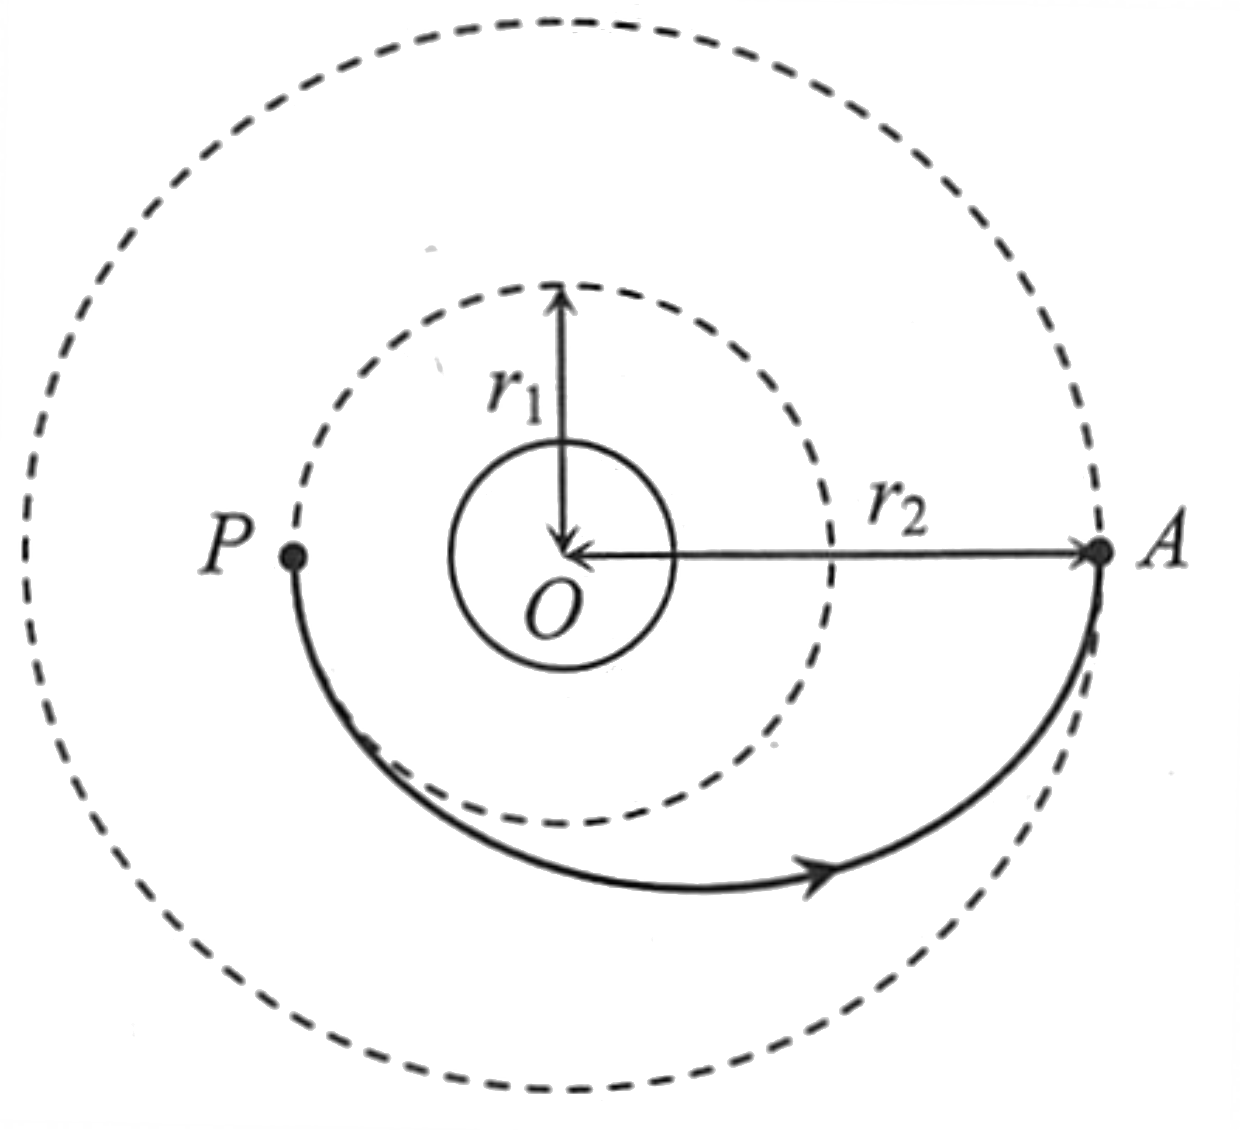
\includegraphics[width=\linewidth]{chgmt_orbite-plain_white}
    \end{center}
\end{minipage}
\begin{rdefi}{Données}
    $M_{\rm Terre} = \SI{5.97e24}{kg}$~; $\Gc = \SI{6.67e-11}{SI}$.
\end{rdefi}

\begin{enumerate}
    \item Calculer la vitesse $v_1$.
    \item Donner l'expression de l'énergie mécanique du satellite sur chacune
        des trois orbites, en fonction de $r_1$ et $r_2$.
    \item Calculer la vitesse $v_{e1}$ après le premier transfert, et la
        variation $\D v_P = v_{e1}-v_1$. Calculer également le travail $W_P$
        fourni par le moteur au satellite en ce point.
    \item Déterminer une relation entre $v_{e1}$, $v_{e2}$, $r_1$ et $r_2$.
        Calculer $v_{e2}$.
    \item Calculer la variation de vitesse $\D v_A = v_2 - v_{e2}$ lors du
        second transfert, ainsi que le travail $W_A$ fourni par le moteur au
        satellite.
\end{enumerate}

% Alerte à l'astéroïde
% Modèle de Bohr
% Expérience de Rutherford

\end{document}
